%%Introduction

%=================================
%%Reference
%%https://www.scribbr.com/research-paper/research-paper-introduction/
%%State the objectives of the work and provide an adequate background, avoiding a detailed literature survey or a summary of the results.

%Step1. Introduce your topic.
     %This is generally accomplished with a strong opening hook.
%Step2. Describe the background.
     %For a paper describing original research, you’ll instead provide an overview of the most relevant research that has already been conducted.
%Step3. Establish your research problem.
     %In an empirical research paper, try to lead into the problem on the basis of your discussion of the literature.
%Step4. Specify your objective(s).
     %The research question is the question you want to answer in an empirical research paper. If your research involved testing hypotheses, these should be stated along with your research question.
%Step 5: Map out your paper.
     %The final part of the introduction is often dedicated to a brief overview of the rest of the paper.
%=================================

The emergence of computer-aided design and digital fabrication could herald a resurgence of intricate and ornate architectural design within our societal fabric, potentially offering a remedy to the uniformity plaguing today's urban landscapes.

Yet, a pivotal question arises: Is contemporary society prepared to once again embrace the realms of ornamentation and complexity, following decades of architectural adherence to the guiding principle of ``form follows function''\cite{Gage2015}, which still wields significant influence over contemporary architectural practices?

The trajectory of history offers insights into this inquiry.
As we delve into the annals of influential architectural styles a compelling pattern unfurls—a dynamic oscillation between the realms of simplicity and complexity (Figure\ref{fig:TimelineArchitecture}).
This enduring pattern is a testament to the interplay between societal values and transformative technological advancements.
%% Figure Timeline Architecture Image
     \begin{figure}[htb]
          \centering
          % trim=left 190 down 250 right 150 top5
          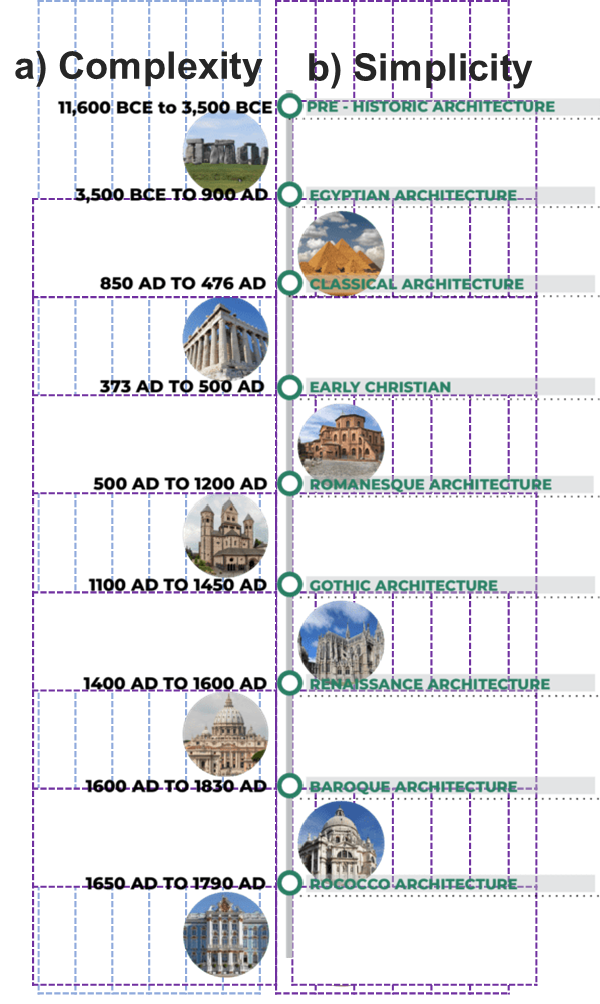
\includegraphics[width= \linewidth]{Images/TimelineArchitecture}
          \caption{Timeline of Architecture and the recurrent pattern of complexity and simplicity}
          \label{fig:TimelineArchitecture}
        \end{figure}

Consider, for instance, the transition from the Romanesque style of the 10th century to the intricate complexity of the Gothic style that flourished in the 14th century\cite{Arora2023}(see Figure\ref{fig:RomanesquevsGothic}).
%%Figure Romanesque vs Gothic figure
     \begin{figure}[htb]
          \centering
          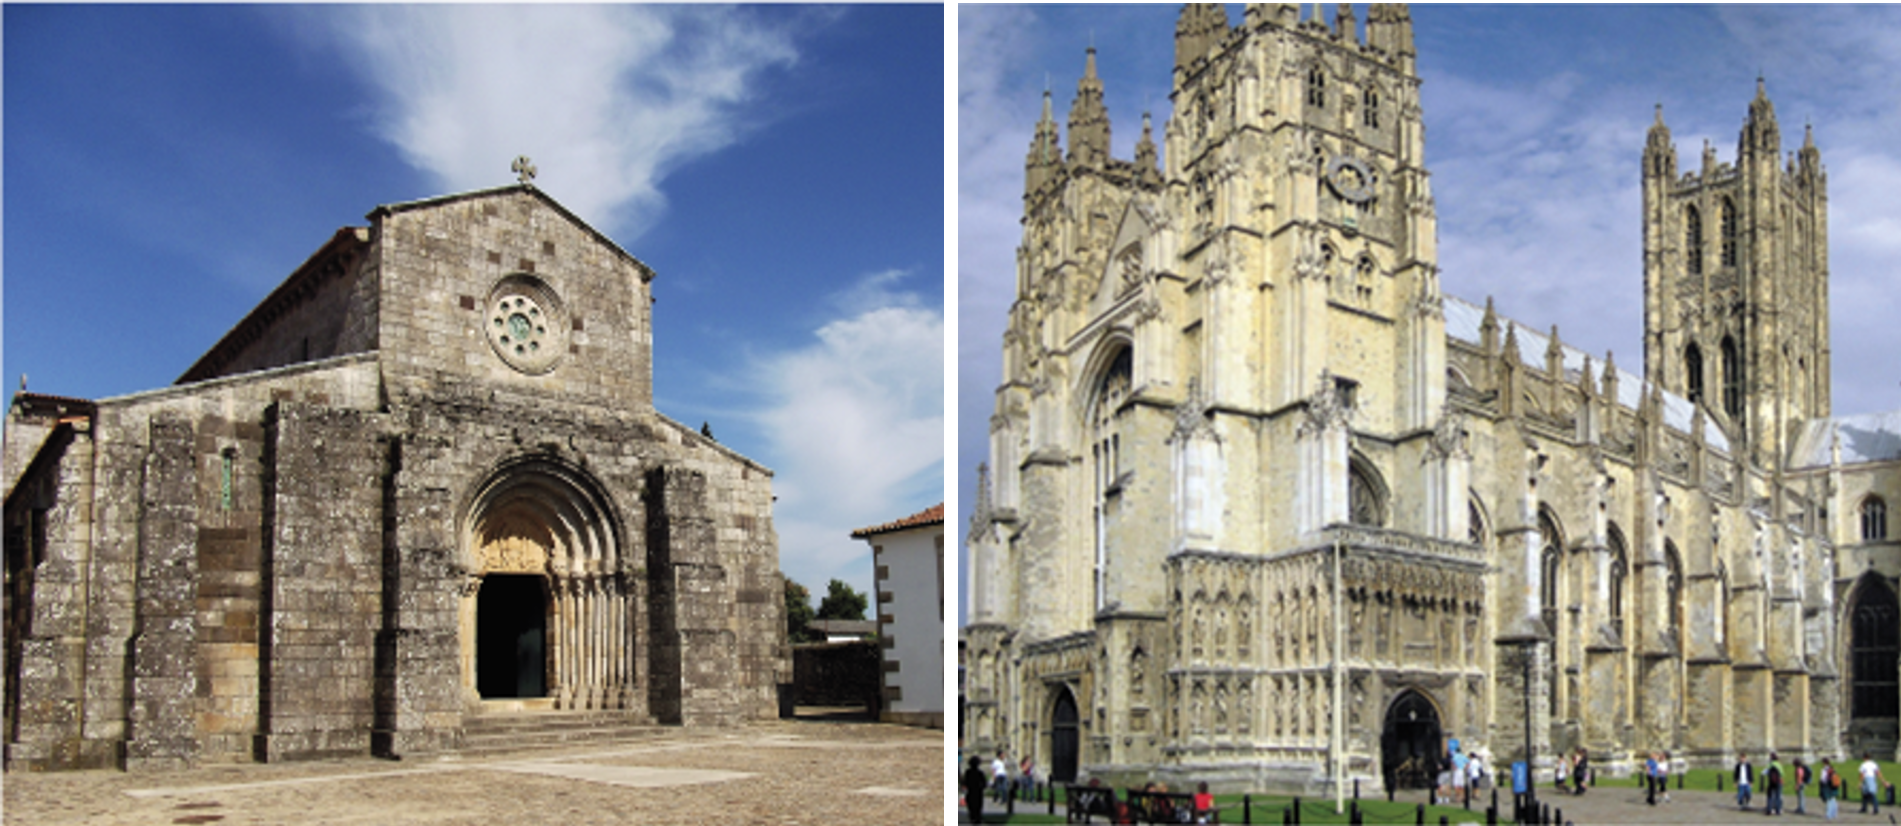
\includegraphics[width= \linewidth]{Images/RomanesqueVsGothic}
          \caption{Romanesque Church 10th AC (left) vs Gothic church 12th AC (right). From simplicity to complexity. (\textit{Images edited from source})}
          \label{fig:RomanesquevsGothic}
        \end{figure}
Similarly, the elaborate Art Deco architecture of the 1920s stands in stark contrast to the subsequent embrace of simplicity of Modern Architecture and rationalism  of the mid-20th century that championed functionalism and minimalist aesthetics, showcasing innovative materials like steel, glass, and concrete\cite{Stacbond2020}(see Figure\ref{fig:ArtNouveauVsModernism}).

%%Figure ArtNouvau vs Modernism
     \begin{figure}[htb]
          \centering
          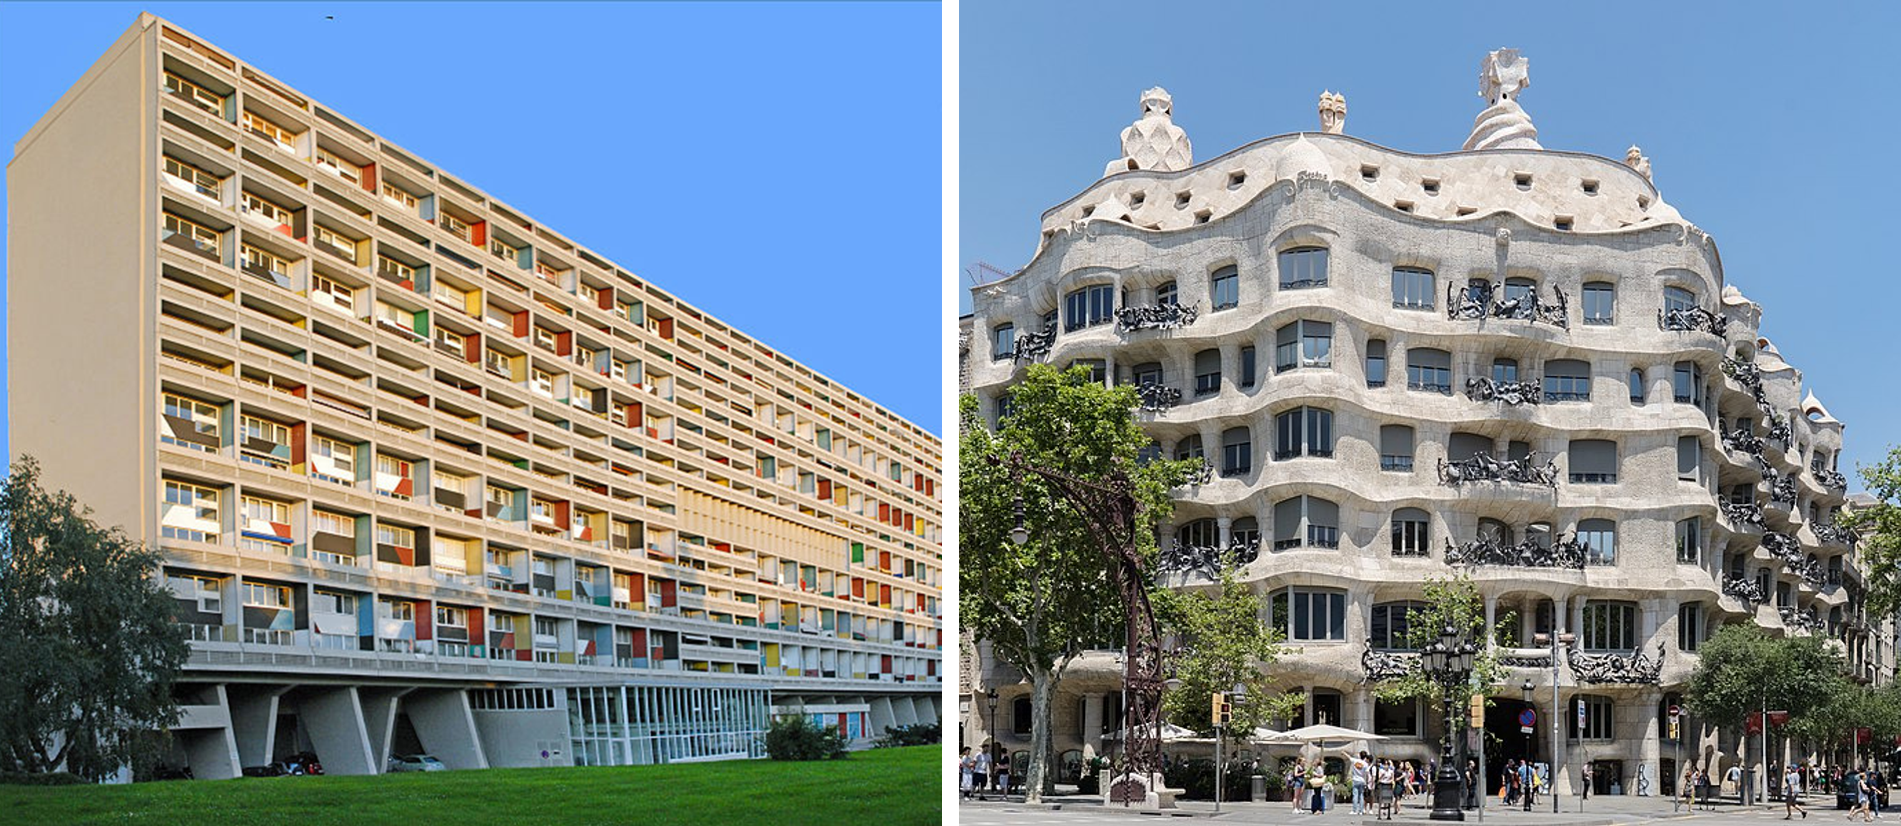
\includegraphics[width= \linewidth]{Images/ArtNouveauVsModernism}
          \caption{Modern Architecture 20th century (Left) vs Art Nouveau building 1920's 30's (Right). To simplicity from complexity. (\textit{Images edited from source})}
          \label{fig:ArtNouveauVsModernism}
        \end{figure}

This shift encapsulates the essence of architectural evolution—an ever-changing interplay between simplicity and complexity, often steered by the confluence of societal values and technological breakthroughs.

Once again, we find ourselves at a pivotal juncture in history, as the emergence of computer-aided design converges with the industrialization of construction, ushering in a new paradigm in architectural design.

In response to the prevailing state of monotonous, one-size-fits-all building design, this paper embarks on an exploration—a quest to reintroduce ornamentation and identity to our urban spaces by embracing the fusion of digital fabrication.

We believe that by harnessing the limitless potential of digital fabrication technology, architecture can rise above the constraints of mass production and rediscover its intricate and inspiring origins, while ensuring that the results remain compelling and well-received by users.

Amidst this transformative pursuit, the advent of mixed reality technology offers a portal to vividly convey the vision of future architectural design.
Immersing stakeholders in a virtual realm where digital fabrication converges with artistry and functionality, a shared understanding of the virtues of complexity can be nurtured.

Through this immersive experience, stakeholders gain firsthand insight into the reimagining of conventional construction methods, especially as the democratization of 3D printing houses and other digital fabrication techniques looms on the horizon.

In this context, this research aims to explore  how users respond to complex facades crafted through  digital fabrication techniques.
Through the medium of a mixed reality experiment, the study seeks to refine our comprehension of complex Facade Design.

By delving into this user-centric exploration,  the research aims to uncover potential interconnections between these insights and predictions related to Future Construction Trends.

In doing so, this study aspires to unravel the intricate web that links user preferences, architectural design intricacy, and the trajectory of forthcoming construction practices.

Hence, this research sets out to address a pivotal question: What degree of complexity and pattern arrangement within facade design, generated through a data-driven design process tailored for digital fabrication, would users tolerate and accept for a building?

The hypothesis posits that participants, regardless of their professional backgrounds and preexisting knowledge of facade design, would provide the essential data needed to refine our grasp of complex facade design through engagement in a Mixed Reality experiment (MR).

Moreover, this data would lay the groundwork for predicting whether the shift towards intricate ornamentation will indeed shape the future trends of construction, as evidenced by the configurations they contribute.

By embracing complexity and transcending the boundaries of mass-produced uniformity, we embrace an opportunity to infuse renewed vibrancy into urban environments, rekindling the spirit of ornamentation and identity, and fostering a sustainable aesthetic inspired by the magnificence of the natural world.

        
%I want to include more references on the timeline

               %Traditionally, it was used to describe the impor- tance of a building revealing its structural system (the form  follows the function of the structure

               %The  idea that we live our lives on a layer of invisible equipment  has significant ramifications for architecture, a discipline that  produces the equipment on and in which we exist.

               %Heidegger's tool analysis posits that while a tool is func- tioning, or its function is visible, the mind registers it as  equipment and, as such, it is rendered invisible to our atten- tion

               %philosophical realism , that is, the belief that there  is a reality outside of the mind, as opposed to philosophical  idealism , which holds that reality exists primarily as a mental  construct.

                %A reaction against 20th-century continental  anti-realism , object-oriented ontology (OOO

%The advent of computer Aid design paired with the already established industrialization of construction, brought in during the creation of the rationalism movement on the 20th century, has provoked a new paradigm shift in the architecture design. The cult of the oversimplification and the ideas of functionality brought by their most canonical representative "Le Corbusier" that birthed cities alienated from the human centric design that had created urban spaces and society \cite{Stacbond2020} in favor for minimalistic approches following an industrial design that ppointed to the machine as the new model for building design \cite{Economakis2023}

%I want to describe the opportunity to bring back ornament and identity to the urban space and buildings by the integration of digital fabrication. as a response to the one size fits all state of current building design that stills considers above all eficiency.

%Also do a quick timeline of the progress of styles or evolution of paradigm in architecture throughout history with the purpose of showing how simplicity follows Images and how society responds in a bit of a cyclical way to it.

%talk about biomimetics too since might be a comunion between performance and aesthetics while contextualizing architecture.

%mention the oportunity of mixed reality to convey all this information to the stakeholders so that they can feel the advantages of great design with the empowering tools of digital fabrication that could reshape the very understanding of common construction with the soon to come democratization of 3d printing houses and other digital fabrication techniques.

%%%%%% Start of text